\chapter{Implementare}

Implementarea aplicației a avut loc în două etape. În prima etapă a fost dezvoltat serverul, care oferea serviciile necesare pentru funcționarea aplicației. În a două etapă a fost dezvoltată aplicația mobilă, care folosește serviciile oferite de server pentru a oferi funcționalitatea necesară utilizatorului final. O dată cu dezvoltarea aplicației, au fost modificate și adăugate noi funcționalități serverului, pentru a oferi noi funcționalități care nu se aflau inițial în cerințele proiectului.
Pe parcursul implementării, au fost folosite diferite tehnologii și servicii externe, actuale și moderne, care au permis dezvoltarea unei aplicații robuste și scalabile. În continuare, sunt prezentate tehnologiile folosite, precum și modul în care au fost folosite.

\section{Sericii externe}

Pentru dezvoltarea aplicației, au fost folosite diferite servicii externe, in special cele oferite de Google pe partea de navigare. Am preferat folosirea unor servicii externe, deoarece acestea oferă funcționalități complexe, care ar fi necesitată o perioadă mai lungă de timp pentru a fi implementate si nu a fost scopul proiectului de a dezvolta aceste funcționalități. De asemenea, aceste servicii sunt oferite de companii mari, care oferă suport și actualizări constante, ceea ce asigură o aplicație robustă și sigură.

\newpage

\subsection{Google Maps Platform}

\begin{wrapfigure}[22]{r}{0.4\textwidth}
    \centering
    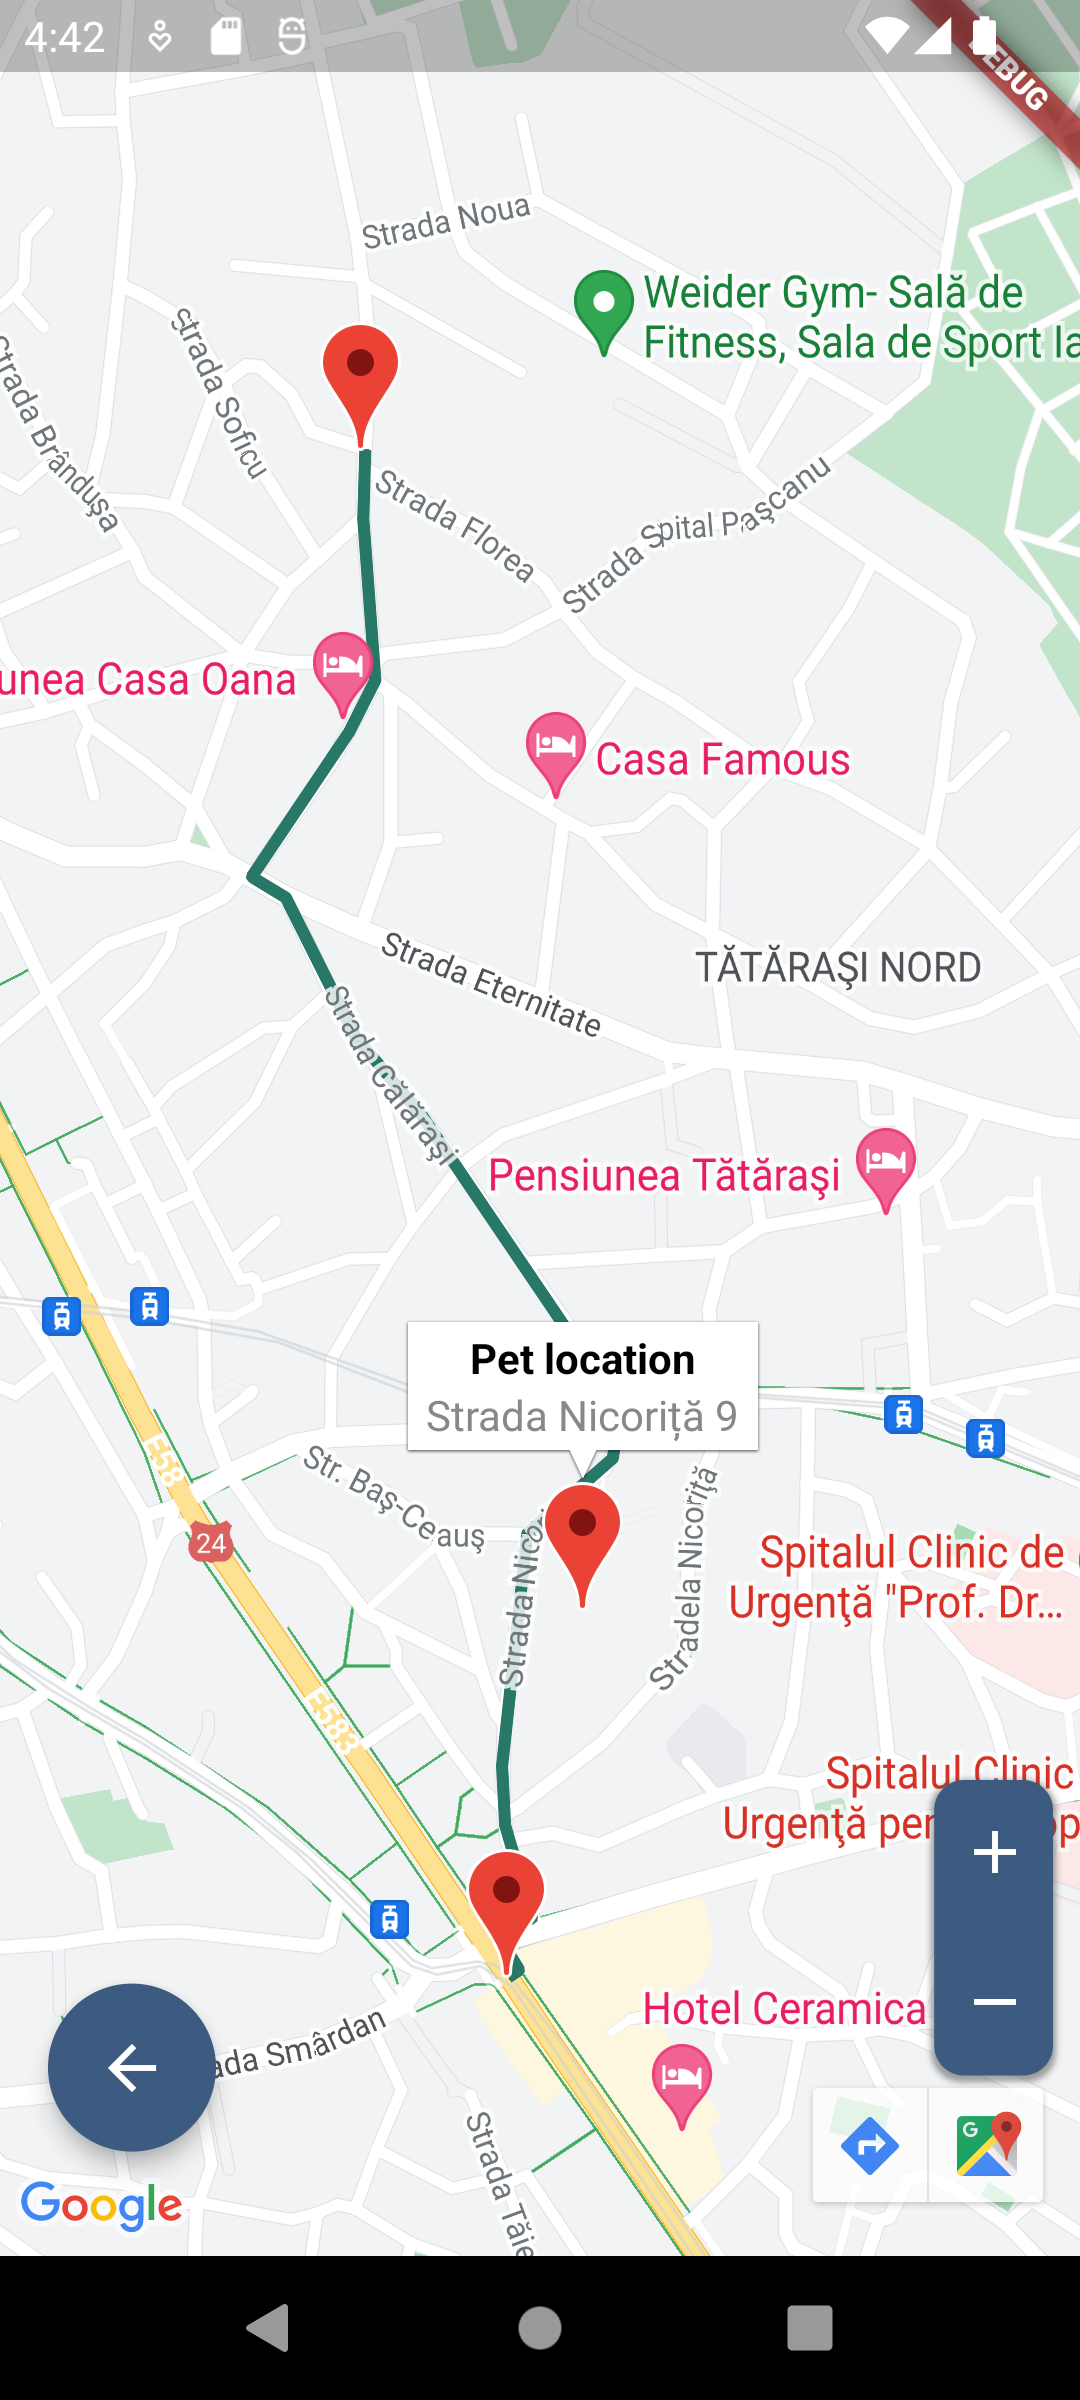
\includegraphics[width=0.4\textwidth]{images/application_map_view.png}
    \caption{Vizualizarea hărții în cadrul aplicației}
    \label{fig:application_map_view}
\end{wrapfigure}

Pentru a putea oferi funcționalitatea de navigare, am folosit serviciul Google Maps. Acesta oferă funcționalitatea de a afișa harta bine cunoscută din cadrul aplicație „Google Maps” și de a calcula și afișa rute între două puncte de pe harta. Pentru a putea folosi serviciul, a fost necesar crearea unui cont de dezvoltator și generarea unei chei de autentificare. Această cheie este folosită de aplicație pentru a se autentifica în cadrul serviciul Google Maps și pentru a putea folosi serviciile oferite de acesta. 
Din cadrul serviciului Google Maps, au fost folosite următoarele servicii:

\begin{itemize}
    \item \textbf{Maps SDK} - 
    oferă funcționalitatea de a afișa harta pe dispozitivul mobil. Acest serviciu este folosit pentru a afișa harta în cadrul aplicației. Harta conține pe lângă străzi și clădiri, și punctele de interes, precum parcuri, restaurante, etc.    
    \item \textbf{Directions API} - oferă funcționalitatea de a calcula rute între două puncte. Acest serviciu este folosit pentru a calcula rutele dintre locația curentă a utilizatorului și locația unde se află animalul de companie, sau pentru a calcula rutele dintre locația animalului de companie și locația unde se află salonul sau cabinetul veterinar.
\end{itemize}

\begin{itemize}
    \item \textbf{Distance Matrix API} - oferă funcționalitatea de a determina distanțele și timpii de parcurgere a drumului dintre două puncte. Acest serviciu este folosit pentru a ajută utilizatorul să estimeze timpul necesar pentru a ajunge la locația unde se află animalul de companie, sau pentru a ajunge la locația unde se află salonul sau cabinetul veterinar pentru o mai bună planificare a timpului.
\end{itemize}

\subsection{Geolocator}

Am utilizat acest servici pentru a determina locația curentă a utilizatorului și ne permite să urmărim locația acestuia pe hartă în momentul deplasării. 

Geolocator oferă posibilitatea de a determina locația curentă a utilizatorului folosindu-se de GPS, rețele mobile și conexiuni WiFi. Acesta poate urmării locația utilizatorului în timp real, oferind informații despre locația curentă, viteza de deplasare, altitudine, etc. Acest serviciu este util atât „Walker” pentru vizualizarea în timp real a drumului pe care îl mai are de parcurs până la destinația curentă cât și „Owner” pentru a spori gradul de siguranță al animalului de companie.

\section{Implementarea serverului}

